\subsubsection{Users}
\def\arraystretch{2}
\begin{table}[H]
\centering
\begin{tabular}{|l|l|}
\hline
Model & User \\ \hline
Controller & UsersControllers \\ \hline
View & Users \\ \hline
Requisiti & ROP 14, ROP 15, ROP 16, RFP 18, ROO 19, ROO 20, ROO 21 \\ \hline
\end{tabular}
\caption{Tracciamento componente-requisiti Users}
\end{table}
Questa componente si occupa della gestione degli utenti, dagli amministratori di OSS agli operatori. Con l'estensione di OSS si andrà ad aggiungere anche il personale delle strutture.
Dato che il sistema OSS verrà reso accessibile anche all'esterno della rete \net si è obbligati a rispettare le direttive sulla privacy. Per questo sono stati aggiunti il campo email e il campo approvato nella relativa tabella del database  e la possibilità di recuperare autonomamente la password persa. Vi è inoltre l'obbligo di modificare la password ogni tre mesi in quanto il sistema contiene \glossario{dati personali} (Ma non \glossario{dati sensibili}).
Quest'ultima funzionalità è già implementata.

\begin{table}[H]
\centering
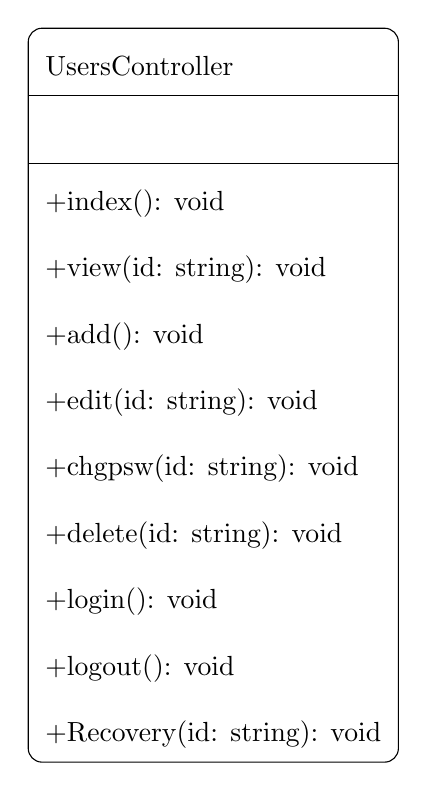
\begin{tikzpicture}
\node (table) [inner sep=0pt] {
\begin{tabular}{l}
  {UsersController} \\
  \hline
  \\
  \hline
  +index(): void \\
  +view(id: string): void  \\
  +add(): void \\
  +edit(id: string): void \\
  +chgpsw(id: string): void \\
  +delete(id: string): void \\
  +login(): void \\
  +logout(): void \\
  +Recovery(id: string): void  \\
\end{tabular}
};
\draw [rounded corners=.5em] (table.north west) rectangle (table.south east);
\end{tikzpicture}
\caption{Controller:UsersController}
\end{table}



\paragraph{Diagrammi delle attività}


\subparagraph{Login}
Di seguito è presentato il diagramma delle attività riguardante l'autenticazione a OSS. I soggetti di tali azioni sono operatori e personale.\\

\begin{figure}[H]
\centering
\includegraphics[width=0.8\textwidth]{images/user_login.png}
\caption{Diagramma attività: Login}
\end{figure}

\textit{Note:}
Il processo di autenticazione esiste già, devono però essere apportate le seguenti modifiche:
\begin{itemize}
\item Nella view va aggiunto un link per il recupero password, che chiamerà il metodo rcvpsw;
\item L'autenticazione dovrà verificare oltre alla corrispondenza username/password anche se tale utente è attivo, controllando se il flag "approvato" è impostato a 1. Questo è possibile farlo aggiungendo l'elemento scope all'array che imposta le opzioni del componente Auth in AppController.php.
\end{itemize}

\label{hash} CakePHP offre la crittazione tramite hash con algoritmo \glossario{MD5}, SHA1, \glossario{SHA256} e blowfish. Attualmete viene utilizzato MD5. Va tenuto presente però che al momento OSS è un software interno mentre dopo l'espansione verrà reso accessibile anche all'esterno. Per tale motivo il tirocinante suggerisce di passare ad una crittazione più forte come SHA-256, comunque supportata nativamente da CakePHP. Inoltre il passaggio sarà effortless per gli utenti in quanto ogni 6 mesi è obbligatorio il cambio password, e proprio in questa occasione si cambierebbe l'algoritmo.


\subparagraph{Recupero password}
Di seguito è presentato il diagramma delle attività riguardante il recupero password. I soggetti di tali azioni sono operatori e personale.\\


\begin{figure}[H]
\centering
\includegraphics[width=0.6\textwidth]{images/user_rcvpsw.png}
\caption{Diagramma attività: Recupero password}
\end{figure}

\textit{Note:}
Il sistema non prevede la possibilità di recupero password, si tratta quindi di una nuova funzionalità. Quando l'utente richiede di recuperare la password:
\begin{itemize}
\item Il sistema genera una passoword casuale di 8 caratteri;
\item Il sistema cripta la passowrd generata con l'algoritmo scelto e salva l'output nel campo password relativo all'utente;
\item Il sistema invia una email con la password all'utente;
\item Nel frattempo l'utente è stato reindirizzato alla pagina di login dove un'avviso gli comunica di controllare la propria casella email;
\item L'utente utilizza la password ricevuta per autenticarsi.
\end{itemize} 


\subparagraph{Nuovo utente}
Di seguito è presentato il diagramma delle attività riguardante la creazione di un nuovo utente. I soggetti di tali azioni sono personale e l'amministratore di OSS.\\

\begin{figure}[H]
\centering
\includegraphics[width=0.6\textwidth]{images/user_new_user.png}
\caption{Diagramma attività: Creazione nuovo account}
\end{figure}


\paragraph{Mokup View}
Di seguito un mockup dell'interfaccia utente per la creazione di un nuovo utente.
I mockup di tutti gli altri casi non vengono creati in quanto banali.
\begin{figure}[H]
\centering
\includegraphics[width=0.3\textwidth]{images/mockup_nuovo_utente.png}
\caption{Mockup nuovo utente}
\end{figure}



% \subsubsection{Rdocumentos}
% \def\arraystretch{2}
% \begin{table}[H]
% \centering
% \begin{tabular}{|l|l|}
% \hline
% Model & Rdocumento \\ \hline
% Controller & RdocumentosControllers \\ \hline
% View & Rdocumentos \\ \hline
% Requisiti &  \\ \hline
% \end{tabular}
% \caption{Tracciamento componente-requisiti}
% \end{table}
% L'operatore del call è loggato ed inizia la vendita della PadovaCard. La prima parte dell'operazione resta invariata, l'operatore crea un nuovo documento e seleziona un cliente; se il cliente è nuovo va a creare l'anagrafica, quindi seleziona l'anagrafica appena creata.
% Il secondo passo è molto simile a quanto viene già fatto, 

% Il processo descritto è suddiviso in due controller, Tdocumentos e Rdocumentos, il primo va a controllare la testata del documento, ovvero l'intestazione, mentre il secondo le righe che compongono tale documento. 

% \textit{Note:} Dal punto di vista dell'usabilità conviene sostituire il menu a tendina da cui sono selezionati ora i clienti con un campo di testo in cui l'operatore può digitare le iniziali del nome o cognome dell'utente e ricevere in tempo reale un feedback degli utenti presenti che corrispondono a tali iniziali.

% \begin{table}[H]
% \centering
% \begin{tikzpicture}
% \node (table) [inner sep=0pt] {
% \begin{tabular}{l}
%   {UsersController} \\
%   \hline
%   \\
%   \hline
%   +totaledoc(id: string): void \\
%   +totaledoccdc(id: string): void \\
%   +totaleoperatore(id: string): void \\
%   +chiusura(id: string, ricevuta: string): void \\
%   +index(): view \\
%   +view(id: string): void \\
%   +add(codice: string): void \\
%   \hline
% \end{tabular}
% };
% \draw [rounded corners=.5em] (table.north west) rectangle (table.south east);
% \end{tikzpicture}
% \caption{Controller:RController}
% \end{table}


% \paragraph{Diagrammi delle attività}


% \subparagraph{Acquisto PadovaCard via call center}
% Di seguito è presentato il diagramma delle attività riguardante l'acquisto PadovaCard via call cente.\\

% \begin{figure}[H]
% \centering
% \includegraphics[width=0.8\textwidth]{images/call_center.png}
% \caption{Diagramma attività: Acquisto PadovaCard via call center}
% \end{figure}

% \paragraph{Mokup View}\label{mockupcallcenter}
% Di seguito un mockup dell'interfaccia che utilizzeranno gli operatori per selezionare le PadovaCard da vendere. Lo step precedente, selezione cliente è già presente e non va modificata, cosi come la sezione successiva di riepilogo e pagamento.
% \begin{figure}[H]
% \centering
% \includegraphics[width=0.5\textwidth]{images/mockup_call_center.png}
% \caption{Mockup selezione PadovaCard}
% \end{figure}




\subsubsection{Tdocumentos}
\def\arraystretch{2}
\begin{table}[H]
\centering
\begin{tabular}{|l|l|}
\hline
Model & Tdocumento \\ \hline
Controller & TdocumentosControllers \\ \hline
View & Tdocumentos \\ \hline
Requisiti & ROU 2, ROU 3, ROU 4, ROU 5, RFU 12, ROO 23, ROO 24, ROS 26 \\ \hline
\end{tabular}
\caption{Tracciamento componente-requisiti Tdocumentos}
\end{table}

La vendita di un qualsiasi articolo, PadovaCard compresa, al momento inizia da questo controller, con la creazione di un nuovo documento e l'associazione dell'anagrafica di un cliente. \\

Di seguito viene descritto il processo di vendita della PadovaCard attuale:
\begin{itemize}
\item L'operatore seleziona "Nuovo Documento";
\item L'operatore seleziona un anagrafica cliente, o la crea se non esiste;
\item L'operatore sceglie quale PadovaCard vendere e vi associa un periodo di validità;
\item La vendita si conclude con il pagamento.
\end{itemize}
Mentre con il nuovo sistema il processo di vendità diventerà:
\begin{itemize}
\item Da \tlite viene generato un file di testo, come descritto nella Sezione \ref{progettazionetlite};
\item L'operatore seleziona "Nuova Padova Card";
\item Il file di testo \tlite corrispondente viene caricato;
\item Il sistema ne estrae i seguenti dati:
	\begin{itemize}
		\item Anagrafica del cliente;
        \item Codice operatore;
        \item Codice cassa;
        \item Codice \tlite;
        \item Elenco di data e ora delle varie visite.
	\end{itemize}
\item 
\item L'operatore associa ad ogni visita un pacchetto, un nominativo e una data/ora di inizio validità;
\item Il sistema verifica che tale data comprenda al suo interno la visita alla \cappella;
\item L'operatore visualizza il totale e lo comunica al cliente che decide il metodo di pagamento;
\item Con carta di credito la vendita viene conclusa e il sistema invia all'utente inserito su \tlite una mail contenente i voucher e tutti i dati necessari.
\item Con bonifico bancario il sistema invierà una email all'utente specificando i dati per il pagamento, quindi quando il pagamento è stato fatto\footnote{Gli operatori controllano quotidianamente gli estratti conto del conto corrente} la carta viene spuntata come attiva.
\end{itemize}

\textit{Note:}\\ \\
\textbf{Caricamento del file testuale}\\

Vi sono due possibilità, caricamento manuale o automatico.\\
Con il caricamento manuale è l'operatore che dopo aver cliccato su "Nuova Padova Card" dovrà cliccare su "Carica File" quindi selezionare il file corretto.
Il sistema controllerà che la data di creazione del file non sia troppo precedente alla data di apertura (10 minuti). \\

Con il caricamento automatico quando l'operatore clicca su "Nuova Padova Card" e quindi su "Carica File" ma è OSS che accede alla cratella in cui si trovano i file, carica tutti i files presenti quindi carica i dati del file di proprietà dell'operatore\footnote{All'interno del file c'è sia il codice operatore che il codice cassa, che sarà confrontato con la login di OSS.}. Una volta caricati i dati su OSS il file viene spostato in una cartella diversa che sarà utilizzata come storico.\\ 

In entrambi i casi è possibile non caricare nessun file, se non vi è nessuna prenotazione da associare, cliccando sul tasto "avanti". Dato che si tratta di un eccezzione alll'operatore verrà chiesto di confermare che si vuole procedere senza caricare nessun file.\\

Si è deciso di utilizzare il caricamento automatico.\\ \\
\textbf{Come vengono estratti i dati dal file} \\ 
Da definire.\\ \\ %TODO
\textbf{Selezionare la PadovaCard} \\

Dalla tendina dei titoli si seleziona una PadovaCard scegliendo tra:
\begin{itemize}
\item 48 ore adulto;
\item 48 ore adulto + minore di 14 anni;
\item 72 ore adulto;
\item 72 ore adulto + minore di 14 anni.
\end{itemize}
Tale scelta deve corrispondere al tipo di prenotazione effettuata su \tlite per la \cappella. Se l'utente vuole una PadovaCard senza \cappella l'operatore sceglierà tra 48/72 ore adulto.
Il passo successivo è scegliere da un altra tendina il pacchetto desiderato, che come visibile dalla figura \ref{mockupperfezionamento} sono suddivisi tra pacchetti base e pacchetti personalizzati.\\ \\
\textbf{Funzionamento del pagamento} \\

Da definire\\ \\ %TODO
\textbf{Informazioni in possesso dell'utente al termine del processo} \\

L'utente la cui anagrafica è stat recuperata dal file \tlite è l'unico di cui si conosce l'email, pertanto sarà lui il destinatario della mail contenente le informazioni. Tale mail la cui veste grafica è visible nell'Appendice %TODO 
conterrà le seguenti informazioni:
\begin{itemize}
\item Anagrafica del cliente;
\item Numero di PadovaCard acquistate;
\item Totale pagato;
\item I voucher di ogni PadovaCard, ognuno composto da:
	\begin{itemize}
		\item Codice a barre della PadovaCard;
        \item Codice a barre di \tlite;
        \item Strutture visitabili con il pacchetto scelto;
        \item Data e ora della visita alla \cappella (Se presente).
	\end{itemize}
\end{itemize}
\textbf{Informazioni in possesso del sistema al termine del processo} \\

Il sistema possiede all'interno della cartella utilizzata come storico i file testuali generati da \tlite. Inoltre una copia dell'email che viene spedita all'utente viene spediata ad un'apposita casella postale di \net. \\

All'interno del database è salvato il log delle operazioni nella tabella log, la transazione nella tabella pagamentos e tutti i datirelativi alla PadovaCard nella tabella cards, consultabile alla Sezione \ref{logicorelazionale}.
\textbf{Possibili errori} \\

Nel caso di caricamento del file manuale potrebbe venir caricato il file errato.
Nel caso in cui le date di attivazione della PadovaCard fossero discordi con le date delle prenotazioni alla \cappella il sistema avverte l'operatore.
Se i nominativi associati alle padovaCard sono errati l'utente se ne accorgerà quando riceve l'email, in tal caso dovrà chiamare nuovamente e far modificare i nominativi errati.\\ 
\textbf{Acquisto di altri articoli allo IAT} \\

Il requisito ROO24 prevede che venga fatto un unico pagamento agli sportelli IAT nel caso in cui l'utente oltre alle PadovaCard acquisti qualcos'altro. Questo è possibile farlo cliccando su "Nuova Riga", visibile sul menu di sinistra nel mockup \ref{perfezionamentoinfo}. Si verrà reindirizzati all'attuale interfaccia di OSS per la vendita.


\paragraph{Diagrammi delle attività}

Di seguito è presentato il diagramma delle attività riguardante il processo di vendita di una PadovaCard. Le versione testuale si trova all'inizio di questa sottosezione. \\
\begin{figure}[H]
\centering
\includegraphics[width=0.6\textwidth]{images/tdocumentos.png}
\caption{Processo di vendita su OSS}
\end{figure}

\paragraph{Mokup View}
Di seguito un mockup della selezione del file e del perfezionamento.
\begin{figure}[H]
\centering
\includegraphics[width=0.6\textwidth]{images/mockup_selezione_file.png}
\caption{Selezione file}
\end{figure}

\begin{figure}[H] \label{mockupperfezionamento}
\centering
\includegraphics[width=0.8\textwidth]{images/mockup_perfezionamento_info.png}
\caption{Perfezionamento delle informazioni\label{perfezionamentoinfo}}
\end{figure}


\subsubsection{Visits}
\def\arraystretch{2}
\begin{table}[H]
\centering
\begin{tabular}{|l|l|}
\hline
Model & Visit \\ \hline
Controller & VisitsControllers \\ \hline
View & Visists \\ \hline
Requisiti & ROU 6, ROP 17, ROS 28 \\ \hline
\end{tabular}
\caption{Tracciamento componente-requisiti Visits}
\end{table}

\begin{table}[H]
\centering
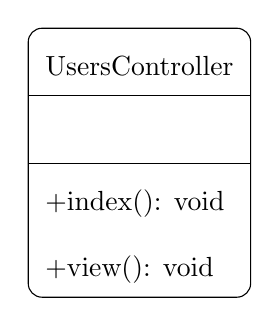
\begin{tikzpicture}
\node (table) [inner sep=0pt] {
\begin{tabular}{l}
  {UsersController} \\
  \hline
  \\
  \hline
  +index(): void \\
  +view(): void \\
\end{tabular}
};
\draw [rounded corners=.5em] (table.north west) rectangle (table.south east);
\end{tikzpicture}
\caption{Controller:VisitsController}
\end{table}
La view collegata ad index corrisponde a quella in figura \ref{validazionecodicebarre}, e permette all'utente di inserire il codice a barre della PadovaCard, manualmente o tramite il lettore.
Il controller index() prende tale valore e recupera le relative informazioni dal database, per poi mostrarle nella view relativa al metodo view. Le informazioni riportate sono:
\begin{itemize}
\item Nome e cognome del possessore della PadovaCard;
\item Data di inizio e fine validità della PadovaCard;
\item Data e ora della visita alla \cappella se si tratta del relativo personale;
\item Validità dell'ingresso, basandosi sul flag "visitato".
\end{itemize}
Dopo aver recuperato le informazioni dal database imposta il flag visitato ad 1, impedendo un ulteriore visita a tale struttura.


\paragraph{Diagrammi delle attività}
Di seguito è presentato il diagramma delle attività riguardante il processo di verifica di validità di una PadovaCard da parte del personale delle strutture.
\begin{figure}[H]
\centering
\includegraphics[width=0.6\textwidth]{images/validazione_padovacard.png}
\caption{Processo di verifica della validità della PadovaCard}
\end{figure}


\paragraph{Mokup View}
Di seguito un mockup delle due viste che ha il personale per validare una PadovaCard.
Notare che il focus per la lettura del codice a barre è già sulla casella di input.
\paragraph{Diagrammi delle attività}
Di seguito è presentato il diagramma delle attività riguardante il processo di verifica di validità di una PadovaCard da parte del personale delle strutture.
\begin{figure}[H]
\centering
\includegraphics[width=0.5\textwidth]{images/mockup_leggi_barcode.png}
\caption{Schermata per la validazione del codice a barre\label{validazionecodicebarre}}
\end{figure}


\subsubsection{Prints}
\def\arraystretch{2}
\begin{table}[H]
\centering
\begin{tabular}{|l|l|}
\hline
Model & Print \\ \hline
Controller & PrintsControllers \\ \hline
View & Prints \\ \hline
Requisiti & ROU 7 \\ \hline
\end{tabular}
\caption{Tracciamento componente-requisiti Prints}
\end{table}

\begin{table}[H]
\centering
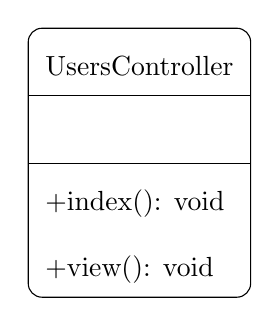
\begin{tikzpicture}
\node (table) [inner sep=0pt] {
\begin{tabular}{l}
  {UsersController} \\
  \hline
  \\
  \hline
  +index(): void \\
  +view(): void \\
\end{tabular}
};
\draw [rounded corners=.5em] (table.north west) rectangle (table.south east);
\end{tikzpicture}
\caption{Controller:PrintsController}
\end{table}
Una PadovaCard può essere stampata solamente agli sportelli IAT, in due occasioni:
\begin{enumerate}
\item L'utente è in possesso del voucher, cartaceo o digitale, ma desidera avere la tessera in cartocnino;
\item L'utente ha smarrito la propria PadovaCard e non è in possesso del voucher, si tratta di un caso meno probabile del precedente.
\end{enumerate}
Nel primo caso all'operatore dello IAT basterà utilizzare il lettore dei codice a barre sul codice del voucher per recuperare i dati, quindi avviare la stampa. \\

Il recupero di una PadovaCard smarrita avviene invece tramite nominativo, per cui l'utente dovrà esibire un documento di riconoscimento all'operatore IAT, il quale recupererà i dati tramite nome e cognome, quindi avvierà la stampa. \\	

La stampa è un semplice bottone che avvia in stampa una PadovaCard sull'apposita stampante.

\paragraph{Mokup View}
Di seguito un mockup della vista che utilizza l'operatore dello IAT per la stampa PadovaCard.
\begin{figure}[H]
\centering
\includegraphics[width=0.5\textwidth]{images/mockup_stampa_tessera.png}
\caption{Schermata per stampa di una PadovaCard\label{stampaPadovaCard}}
\end{figure}


\subsubsection{EditPadovaCard}
\def\arraystretch{2}
\begin{table}[H]
\centering
\begin{tabular}{|l|l|}
\hline
Model & EditPadovaCard \\ \hline
Controller & EditPadovaCardsControllers \\ \hline
View & EditPadovaCards \\ \hline
Requisiti & ROO 25, RFO 31 \\ \hline
\end{tabular}
\caption{Tracciamento componente-requisiti EditPadovaCard}
\end{table}

\begin{table}[H]
\centering
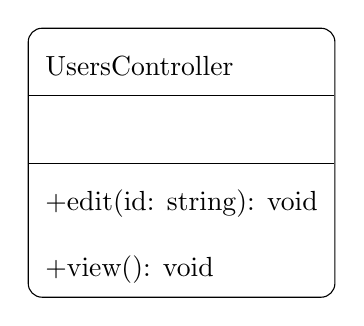
\begin{tikzpicture}
\node (table) [inner sep=0pt] {
\begin{tabular}{l}
  {UsersController} \\
  \hline
  \\
  \hline
  +edit(id: string): void \\
  +view(): void \\
\end{tabular}
};
\draw [rounded corners=.5em] (table.north west) rectangle (table.south east);
\end{tikzpicture}
\caption{Controller:EditPadovaCard}
\end{table}

La view da cui inizia l'operazione di modifica del nominativo o della data di inizio validità della PadovaCard è la stessa utilizzata per la stampa, visibile nella Figura \ref{stampaPadovaCard}. In questo caso dopo aver inserito il codice della PadovaCard o il nominativo invece di cliccare su recupero dati l'ioperatore clicca su modifica dati, che reindirizza su una nuova view da cui sarà possibile apportare le modifiche. I dettagli di questa view sono visibile nella figura \ref{modificaPadovaCard}.

\paragraph{Diagrammi delle attività}
Di seguito è presentato il diagramma delle attività riguardante il processo di modifica della data di validità e del nominativo associati ad una PadovaCard.
\begin{figure}[H]
\centering
\includegraphics[width=0.6\textwidth]{images/modifica_padovacard.png}
\caption{Processo di modifica dati PadovaCard}
\end{figure}

\paragraph{Mokup View}
Di seguito un mockup della vista che utilizza l'operatore per modificare data di validità e nominativo associati ad una PadovaCard.
\begin{figure}[H]
\centering
\includegraphics[width=0.5\textwidth]{images/mockup_modifica_tessera.png}
\caption{Schermata per stampa di una PadovaCard\label{modificaPadovaCard}}
\end{figure}


\subsubsection{Parser}
Il parser sarà scritto in PHP e prenderà in input il file testuale stampato da \tlite, sia caricato manualmente sia automaticamente. L'output del parser sarà un array contenente:
\begin{itemize}
	\item Anagrafica del cliente;
    \item Codice operatore;
    \item Codice cassa;
    \item Codice \tlite;
    \item Elenco di data e ora delle varie visite.
\end{itemize}

Il file in input non avrà sempre la stessa forma in quanto ci sono diversi casi da prendere in considerazione:
\begin{itemize}
\item Acquisto di un singolo ingresso adulto;
\item Acquisto di un singolo ingresso adulto+bambino
\item Acquisto di n ingressi adulto nello steso giorno e stessa fascia oraria;
\item Acquisto di n ingressi adulto+bambino nello steso giorno e stessa fascia oraria;
\item Acquisto di n ingressi adulto/adulto+bambino nello steso giorno e stessa fascia oraria;

\item Acquisto di n ingressi adulto nello steso giorno e diverse fascie orarie;
\item Acquisto di n ingressi adulto+bambino nello steso giorno e diverse fascie orarie;
\item Acquisto di n ingressi adulto/adulto+bambino nello steso giorno e diverse fascie orarie;

\item Acquisto di n ingressi adulto in giorni diversi e diverse fascie orarie;
\item Acquisto di n ingressi adulto+bambino in giorni diversi e diverse fascie orarie;
\item Acquisto di n ingressi adulto/adulto+bambino in giorni diversi e diverse fascie orarie;

\item L'anagrafe del cliente è completa o mancano alcuni parametri.
\end{itemize}
Di seguito un esempio del file che il parser prenderà in input.
\lstset{frame=single}
\begin{center}
\begin{lstlisting}
Ricevuta di Pagamento

                                     Rossi Mario
             Acquistati da    Via Giulio Cesare 01/A 35128 padova (pd) Italia
             
             Codice Transazione                                                      TLITE0528719557735
             
             Evento       Cappella degli Scrovegni e Musei Civici degli Eremitani del 14/05/2015 17:15 
             
             Sala                                                              Cappella degli Scrovegni
             
             Organizzatore                                                             Comune di Padova
             
             Zona                Descrizione posto      Riduzione             N.Bigl.  Prezzo  Prev.
             Ingressi            Ingresso               GRATUITO GUIDE              1    0,00   0,00
             
             Totale ricevuta                                                      1          0,00
             
             Gli importi sono comprensivi di iva
             
             Casse e                                                                         PC-01
             operatore                                                                        OperatoreX 
             
             Pagati da
             
             Data emissione                                                            30/01/2015 12:47
             
             Ritiro biglietti
             E' possibile ritirare i biglietti presso la biglietteria del museo a partire dal giorno 
             seguente all'acquisto. Il ritiro del biglietto deve avvenire con congruo anticipo: si 
             consiglia soprattutto ai gruppi di presentarsi in biglietteria almeno 45 minuti prima 
             dell'orario di visita. In caso di acquisto di riduzioni il personale del museo potra' 
             richiedere documentazione per verificare l'effettiva validita' dell'acquisto. 

\end{lstlisting}
\end{center}
I dati dell'utente si trovano immediatamente sotto la dicitura "RIcevuta di pagamento", il codice \tlite è marcato dalla dicitura "Codice Transazione", data e ora della visita al termine della riga che corrisponde a "Evento" ed infine Cassa e operatore indicano il codice postazione ed il codice dell'operatore  che ha effettuato la vendita.

\subsubsection{Creazione codice a barre univoco}
Il codice a barre utilizzato è presentato nella sezione \ref{codicebarre}. Di seguito è spiegato come il codice viene generato. \\

Si è scelto di utilizzare l'output della funziona hash SHA-256 più due caratteri, che saranno i secondi del timestamp del log dell'operazione di creazione di una nuova PadovaCard. 
L'input utilizzato per la funzione di hash è dato dalla dato dal codice \tlite, più un valore di salt, ovvero una sequenza casuale di bit generata da CakePHP.\\

La funzione SHA-256 prende tale input e lo trasforma in una sequenza di 256 bit, siccome nel nostro database abbiamo dichiarato il campo codicecarta di tipo char(10) esso conterrà al più 80bit, per questo motivo tronchiamo i 256 bit di output a 64, cui andranno aggiunti i 16 bit dei restanti due caratteri.\\ 

Grazie all'aggiunta di questi due caratteri si evita il problema di possibili collisioni di input.

% Per il Principio dei cassetti teoricamente è possibile una collisione, ma attualmente nessuno ha trovato due input che collidano sullo stesso hash utilizzando SHA-256, troncando l'output della funzione teoricamente si diminuisce la sua resistenza alle collisioni, ma in pratica sono ancora necessari 2\textsuperscript{40} tentativi. 


